\chapter{산란, 쌍대성, 그리고 베네치아노 진폭}

\lectureoverview{산란은 충돌을 실험과 비교할 수 있는 불변량으로 나타낸다. 동일한 입자 4개의 경우 이 불변량은 만델스탐 변수 \(s,t,u\)로 정리할 수 있으며, 그중 독립적인 것은 2개뿐이다. 보통 입자 교환을 생각하면 직접 채널과 교차 채널이 따로 있을 것으로 예상된다. 베네치아노 진폭은 이 예상을 뒤집었다. 하나의 함수가 두 채널에 대한 기술을 모두 담고 있다. 강의의 후반부에서는 결합해 하나의 진동하는 사슬로 진화한 뒤 다시 분리되는 두 개의 열린 끈으로부터 이 함수를 구성한다.}

\section{이론이 예측해야 하는 것}

페르미온 끈은 순수 보손 모형의 두 가지 결함을 해결한다. 페르미온 상태를 허용하고, 적절한 사영을 거친 뒤에는 타키온을 제거한다. 임계 시공간 차원은 26이 아니라 10이다. 따라서 여분 차원은 여전히 남지만, 그 콤팩트화는 뒤로 미룬다. 여기서는 우선 산란을 다룬다.
\editorialnote{타키온이 없다는 말은 필요한 사영을 거친 일관된 초끈 스펙트럼을 가리킨다. 세계면 페르미온을 더하는 것만으로는 충분하지 않다.}

입자가 하는 일 가운데 산란이 반드시 가장 흥미로운 것은 아니다. 다만 실험에서 깔끔하게 반복할 수 있는 과정이다. 정해진 입자들을 서로를 향해 보내고, 충돌 뒤에 나오는 입자들을 기록한 다음, 상호작용 영역 내부에 감춰진 동역학을 추론한다. 이론이 복소 진폭 \begin{equation}
  \mathcal A(\hbox{incoming data}\to\hbox{outgoing data}),
\end{equation}을 제시하면 정량적인 이론이 된다. 이 진폭의 절댓값을 제곱하고 통상적인 위상 공간 인자를 곱하면 해당 결과가 나올 확률을 얻는다.

\begin{figure}[H]
  \centering
  
\includegraphics[width=0.72\textwidth]{lecture_06_figure_01.png}
  \caption{입사 입자들이 블랙박스 상호작용 영역으로 들어가고 산란 입자들이 나온다. 시간은 가로 방향으로 표시되어 있다.}
  \lectureframe{00:02:35}
  \label{fig:l06-black-box}
\end{figure}

입자에는 스핀, 전하, 종을 나타내는 표지도 붙어 있다. 먼저 운동학적 성질을 드러내기 위해 운동량 이외의 모든 것은 잠시 무시하자.

\section{사차원 운동량과 전부 입사로 보는 규약}

입자 하나의 사차원 운동량을 다음과 같이 쓰자.
\begin{equation}
  k^\mu=(k^0,\mathbf k)=(E,\mathbf p).
\end{equation}강의에서는 대부분의 부호가 양수인 계량을 사용하므로
\begin{equation}
  k^2\equiv \mathbf p^2-E^2.
\end{equation}상대론적 분산 관계는 따라서 다음과 같다.
\begin{equation}
  E^2-\mathbf p^2=m^2,
  \qquad
  k^2=-m^2.
  \label{eq:l06-mass-shell}
\end{equation}공간 운동량을 바꾸면 에너지는 변하지만, 입자는 질량 껍질을 벗어나지 않는다.

\begin{figure}[H]
  \centering
  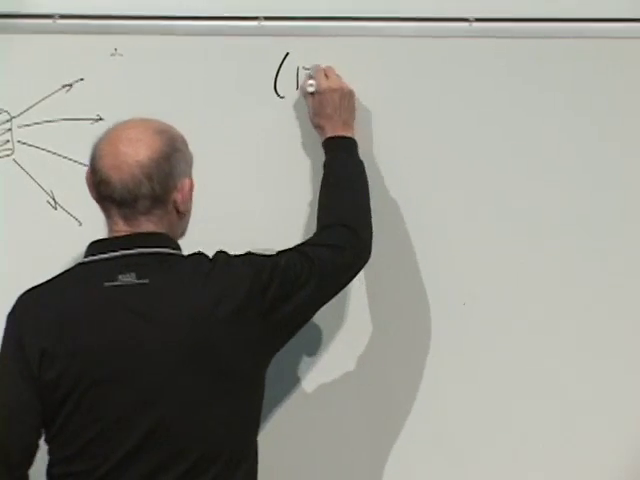
\includegraphics[width=0.66\textwidth]{lecture_06_figure_02.png}
  \caption{강의 전반에서 사용하는 계량 규약에서의 질량 껍질 조건.}
  \lectureframe{00:05:56}
  \label{fig:l06-mass-shell}
\end{figure}

운동량 \(k_1,k_2\)을 가진 입자 두 개가 들어오고, 물리적 운동량 \(q_3,q_4\)을 가진 입자 두 개가 나간다고 하자. 에너지와 운동량의 보존은 하나의 사차원 벡터 방정식으로 표현된다.
\begin{equation}
  k_1+k_2=q_3+q_4.
  \label{eq:l06-physical-conservation}
\end{equation}모든 외부선을 입사 운동량으로 나타내면 편리하다.
\begin{equation}
  k_3\equiv-q_3,
  \qquad
  k_4\equiv-q_4.
\end{equation}그러면
\begin{equation}
  k_1+k_2+k_3+k_4=0,
  \label{eq:l06-all-incoming}
\end{equation}이고 각 다리는 \(k_i^2=-m_i^2\)을 만족한다. 이 장부 기록 규약에서만 산란 입자들의 에너지가 음수로 나타난다. 물리적 에너지는 여전히 양수다.

\begin{figure}[H]
  \centering
  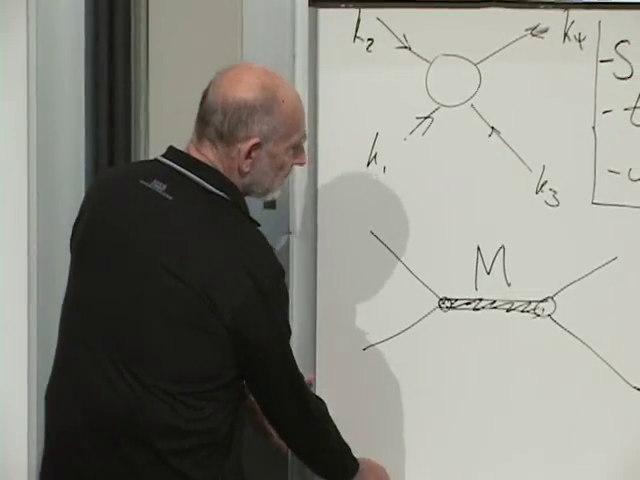
\includegraphics[width=0.68\textwidth]{lecture_06_figure_03.png}
  \caption{네 개의 외부 운동량을 대칭적으로 모두 입사로 다루도록, 물리적 산란 운동량의 방향을 뒤집는다.}
  \lectureframe{00:09:10}
  \label{fig:l06-all-incoming-board}
\end{figure}

처음에는 진폭이 16개의 성분 \(\mathcal A(k_1,k_2,k_3,k_4)\)을 인자로 하는 것처럼 보인다. 하지만 대부분은 중복 정보다. 질량 중심계로 가서 입사 운동량을 선택한 축에 맞추고, 간단히 네 입자의 질량이 모두 같다고 하자. 그러면 입사 상태는 질량 중심 에너지라는 하나의 수로 정해진다. 산란 입자들의 공간 운동량은 크기가 같고 방향이 서로 반대여야 하며, 그 크기는 입사 쌍의 운동량 크기와 같아야 한다. 남는 것은 산란각 \(\theta\)뿐이다. 따라서 이 과정에는 독립적인 운동학적 변수가 두 개 있다.
\begin{equation}
  E_{\mathrm{cm}},
  \qquad
  \theta.
  \label{eq:l06-two-data}
\end{equation}

\section{만델스탐 변수}

\eqref{eq:l06-two-data}에 등장하는 두 물리량은 기준계를 선택하지 않고 표현할 수 있어야 한다. 전부 입사로 보는 규약에 따라 다음과 같이 정의하자.
\begin{equation}
  \begin{aligned}
    -s&=(k_1+k_2)^2,\\
    -t&=(k_1+k_3)^2,\\
    -u&=(k_1+k_4)^2.
  \end{aligned}
  \label{eq:l06-mandelstam}
\end{equation}질량 중심계에서는 \(k_1+k_2\)의 공간 성분들이 상쇄되므로
\begin{equation}
  s=E_{\mathrm{cm}}^2.
  \label{eq:l06-s-energy}
\end{equation}

산란된 물리적 운동량 \(q_3=-k_3\)에 대해,
\begin{equation}
  k_1+k_3=k_1-q_3
\end{equation}는 다리 1에서 다리 3로 전달된 운동량이다. 외부 입자들의 질량이 같고 입사 공간 운동량의 크기가 \(p\)일 때,
\begin{equation}
  -t=2p^2(1-\cos\theta),
  \qquad
  -u=2p^2(1+\cos\theta).
  \label{eq:l06-tu-angle}
\end{equation}따라서 \(t\)와 \(u\)는 검출기로 측정하는 각도 정보를 담는다.

\begin{figure}[H]
  \centering
  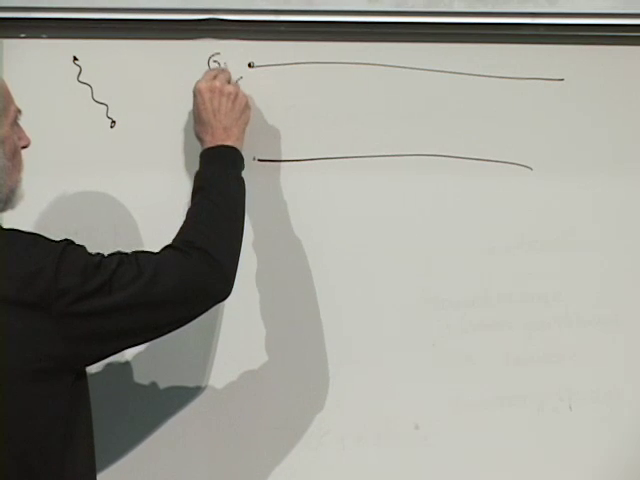
\includegraphics[width=0.74\textwidth]{lecture_06_figure_04.png}
  \caption{전부 입사 규약에서 \(s,t,u\)를 대칭적으로 정의한 식.}
  \lectureframe{00:26:20}
  \label{fig:l06-stu-board}
\end{figure}

기호가 세 개라고 해서 독립적인 정보도 세 가지인 것은 아니다. \eqref{eq:l06-all-incoming}을 제곱하고 \(k_i^2=-m^2\)을 사용하면 질량이 같은 경우
\begin{equation}
  s+t+u=4m^2
  \label{eq:l06-stu-constraint}
\end{equation}을 얻는다. \(s\)과 \(t\)을 알면 \(u\)은 정해진다.

\begin{classroomqa}
\audiencequestion{진공이 마찰처럼 작용해 자유롭게 움직이는 입자를 느리게 할 수 있을까요? \lecturetimestamp{00:27:17}}
\lecturerresponse{병진 대칭인 진공에서는 그럴 수 없습니다. 잃어버린 운동량이 갈 곳이 없으므로 운동량 보존이 그런 마찰을 금지합니다. 매질이나 선호하는 정지 기준계를 정하는 다른 진공을 생각할 수는 있지만, 여기서 다루는 진공은 그런 진공이 아닙니다.}
\end{classroomqa}

\begin{classroomqa}
\audiencequestion{산란된 두 입자의 에너지는 왜 같아야 하나요? \lecturetimestamp{00:27:54}}
\lecturerresponse{질량 중심계에서 두 입자의 공간 운동량은 크기가 같고 방향이 서로 반대여야 합니다. 여기서 다루는 과정처럼 두 입자의 질량이 같으면, 운동량 크기가 같으므로 \(E^2=p^2+m^2\)에 따라 에너지도 같습니다. 산란 입자들의 질량이 서로 다르다면 이 결론은 수정되어야 합니다.}
\end{classroomqa}

\section{직접 채널과 교차 채널}

단순한 점입자 도표에서는 입자 1과 2이 질량 \(M\)인 중간 입자를 만들고, 이 입자가 다시 3과 4로 붕괴할 수 있다. 분자 인자와 극점 처방을 제외하면 이 과정의 특징적인 의존성은 다음과 같다.
\begin{equation}
  \mathcal A_s\sim\frac{g^2}{s-M^2}.
  \label{eq:l06-s-channel}
\end{equation}이는 직접 채널, 즉 \(s\) 채널 과정이다. 연결 관계를 옆으로 돌리면 두 외부선 사이의 교환이 된다.
\begin{equation}
  \mathcal A_t\sim\frac{g^2}{t-M^2},
  \label{eq:l06-t-channel}
\end{equation}이는 교차 채널, 즉 \(t\) 채널 과정이다. 세 번째 연결 관계는 다음과 같다.
\begin{equation}
  \mathcal A_u\sim\frac{g^2}{u-M^2}.
  \label{eq:l06-u-channel}
\end{equation}

\begin{figure}[H]
  \centering
  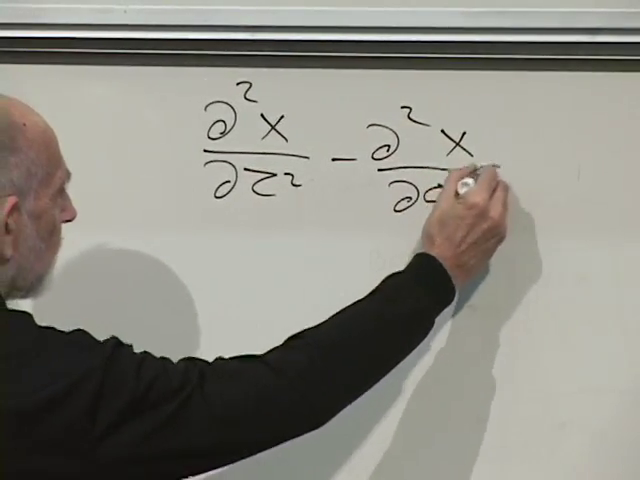
\includegraphics[width=0.72\textwidth]{lecture_06_figure_05.png}
  \caption{중간 상태를 통한 직접 생성과 이에 대응하는 극점 \(g^2/(s-M^2)\). 같은 판 위에 교차 채널의 연결 관계도 구성하고 있다.}
  \lectureframe{00:30:50}
  \label{fig:l06-channel-board}
\end{figure}

이 구분은 물리적이다. 이렇게 조잡한 스칼라 수준에서는 \eqref{eq:l06-s-channel}이 충돌 에너지에는 의존하지만 각도에는 의존하지 않는다. 복합 상태는 붕괴하기 전에 입사 방향에 대한 정보를 잃으므로 붕괴는 등방적이다. 교환 진폭은 운동량 전달에 의존하므로 각도에도 의존한다. 교환 입자의 질량이 작으면 산란각이 작아지는 과정이 강하게 우세해진다. 스핀을 고려하면 각도 의존성이 더 생기지만, 극점 구조는 이미 드러나 있다.

\begin{classroomqa}
\audiencequestion{빠진 \(u\) 채널에서도 세 번째 항이 생기나요? \lecturetimestamp{00:34:47}}
\lecturerresponse{입자의 종류와 결합이 그 연결 관계를 허용하면 생깁니다. 그러면 \(u=M^2\)에 극점을 갖는 항을 포함합니다. \(s+t+u=4m^2\)이므로 이것은 새로운 독립 운동학 변수가 아니지만, 별개의 채널 도표입니다.}
\end{classroomqa}

\section{하나의 함수, 두 가지 채널 기술}

하나의 극점만으로는 중간자 산란을 제대로 설명하기 어렵다. 두 중간자는 질량과 각운동량이 서로 다른 여러 공명 상태를 만들 수 있다. 1960년대에는 우선 \(s\) 채널 극점과 \(t\) 채널 극점을 더하고, 허용되는 \(u\) 채널 극점도 추가하는 방식으로 대응했다. 그러다가 훨씬 간결한 함수가 발견되었다. 선형 레제 궤적과 절편을 \(s\)와 \(t\)에 흡수한 강의의 단위계에서는 다음과 같다.
\begin{equation}
  \mathcal A_{\mathrm V}(s,t)
  \propto
  \frac{\Gamma(-s)\Gamma(-t)}{\Gamma(-s-t)}.
  \label{eq:l06-veneziano}
\end{equation}감마 함수는 양의 정수에서 계승을 일반화한다.
\begin{equation}
  \Gamma(n)=(n-1)!
\end{equation}

\begin{figure}[H]
  \centering
  \includegraphics[width=0.68\textwidth]{lecture_06_figure_06.png}
  \caption{감마 함수들의 대칭적인 비로 쓴 베네치아노 진폭.}
  \lectureframe{00:42:25}
  \label{fig:l06-veneziano-board}
\end{figure}

\(\Gamma(-s)\)의 극점은 무한한 직접 채널 공명 탑을 재현한다. 그런데 같은 식은 \(s\leftrightarrow
t\)에 대해 대칭이므로, \(\Gamma(-t)\)의 극점들은 교차 채널 전개도 제공한다. 이 두 기여를 따로 더한 것이 아니다. 하나의 해석 함수가 두 가지 기술을 모두 허용한다. 이것이 직접 채널 공명과 교차 채널 교환 사이의 오래된 쌍대성 개념이다.

\begin{classroomqa}
\audiencequestion{어떻게 하나의 진폭이 두 채널의 합을 더하지 않고 모두 담을 수 있나요? \lecturetimestamp{00:43:32}}
\lecturerresponse{바로 그것이 놀라운 점입니다. 함수의 \(s\) 채널 극점 근방에서 전개하면 직접 공명들로 정리되고, \(t\) 채널 극점 근방에서 전개하면 같은 함수가 교환 과정들로 정리됩니다. 이 두 해석이 왜 같은지를 설명하려면 미시적 모형이 필요하며, 그 모형이 상호작용하는 끈입니다.}
\end{classroomqa}

\section{열린 끈이 쓸어 만드는 띠}

열린 끈을 다음과 같이 매개화하자.
\begin{equation}
  0\leq\sigma\leq\pi.
\end{equation}표지 \(\sigma\)는 시공간 위치가 아니다. 매장 \(X^\mu(\sigma,\tau)\)은 그 표지가 붙은 점이 시공간의 어디에 놓이는지를 나타내며, \(\tau\)는 시간에 따른 변화를 나타낸다. 점입자가 쓸어 만드는 것은 세계선이고, 움직이는 끈은 2차원 세계면을 쓸어 만든다. 자유 이론에서는 각 매장 좌표가 다음 방정식을 만족한다.
\begin{equation}
  \frac{\partial^2X^\mu}{\partial\tau^2}
  -
  \frac{\partial^2X^\mu}{\partial\sigma^2}
  =0.
  \label{eq:l06-wave-equation}
\end{equation}

\begin{figure}[H]
  \centering
  \includegraphics[width=0.70\textwidth]{lecture_06_figure_07.png}
  \caption{세계면 띠 위에서 각 자유 끈 좌표를 지배하는 파동 방정식.}
  \lectureframe{00:49:10}
  \label{fig:l06-wave-equation-board}
\end{figure}

산란 과정을 구성할 때는 연속체 극한을 너무 일찍 취하지 않는 편이 유용하다. 각 끈을 스프링으로 연결된 질량점 \(n\)개로 바꾸자. 세계면은 서로 가까운 세계선들이 빽빽이 모인 형태가 되고, 정상 모드는 보통의 조화 진동자가 된다. 두 입사 사슬은 끝점에서 맞닿을 수 있다. 그 순간 새 스프링이 두 사슬을 연결해 하나의 더 긴 사슬로 만들고, 그 사슬은 시간 \(\tau\) 동안 진화한다. 나중에 스프링이 끊어지면 산란 사슬 두 개가 나온다.

\begin{figure}[H]
  \centering
  \includegraphics[width=0.72\textwidth]{lecture_06_figure_08.png}
  \medskip

  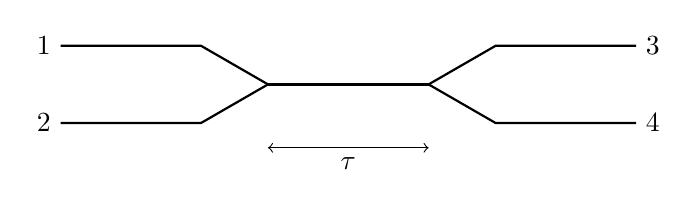
\begin{tikzpicture}[x=0.85cm,y=0.70cm]
    \draw[thick] (0,2.2) -- (2.1,2.2) -- (3.1,1.5);
    \draw[thick] (0,0.8) -- (2.1,0.8) -- (3.1,1.5);
    \draw[thick] (3.1,1.5) -- (5.5,1.5);
    \draw[thick] (5.5,1.5) -- (6.5,2.2) -- (8.6,2.2);
    \draw[thick] (5.5,1.5) -- (6.5,0.8) -- (8.6,0.8);
    \draw[<->] (3.1,0.35) -- node[below] {\(\tau\)} (5.5,0.35);
    \node[left] at (0,2.2) {1};
    \node[left] at (0,0.8) {2};
    \node[right] at (8.6,2.2) {3};
    \node[right] at (8.6,0.8) {4};
  \end{tikzpicture}
  \caption{이산화한 열린 끈 두 개가 맞닿아 하나의 중간 끈을 이루고, 시간 \(\tau\) 동안 지속된 뒤 분리된다. 원본 화면은 스프링과 세계선으로 구성된 그림을 보존하며, 도식은 그 연결 관계를 따로 보여 준다.}
  \lectureframe{00:51:25}
  \label{fig:l06-string-joining}
\end{figure}

두 끈은 매개변수 공간에서만 나란히 그려져 있다. 끝점 좌표가 실제로 일치하기 전까지 두 끈의 시공간 위치는 서로 가까울 필요가 없다. 재매개화 자유도를 이용하면 도표에서 결합과 분리 사건을 편리한 위치에 놓을 수 있다. 이 기하학적 자유도는 다음 강의에서 등각 대칭으로 나타난다.

\section{진동자 계산을 천천히 따라가기}

첫 번째 사슬의 좌표를 \(x_1,\ldots,x_n\), 두 번째 사슬의 좌표를 \(x_{n+1},\ldots,x_{2n}\)라 하자. 두 사슬의 질량 중심 좌표는 다음과 같다.
\begin{equation}
  X_{\mathrm{cm}}^{(1)}
  =\frac1n\sum_{a=1}^{n}x_a,
  \qquad
  X_{\mathrm{cm}}^{(2)}
  =\frac1n\sum_{a=n+1}^{2n}x_a.
  \label{eq:l06-chain-centers}
\end{equation}운동량이 정해진 \(k_1\)을 가진 사슬의 파동함수는 질량 중심 평면파에 내부 진동자의 바닥 상태를 곱한 형태다.
\begin{align}
  \Psi_1
  &=
  e^{ik_1\cdot X_{\mathrm{cm}}^{(1)}}
  \psi_0(x_1,\ldots,x_n),
  \\
  \Psi_2
  &=
  e^{ik_2\cdot X_{\mathrm{cm}}^{(2)}}
  \psi_0(x_{n+1},\ldots,x_{2n}).
  \label{eq:l06-two-wavefunctions}
\end{align}인자 \(\psi_0\)는 상대 좌표에 의존하며, 사슬 전체를 함께 평행 이동시키는 데에는 의존하지 않는다. 입사 끈들은 처음에 서로 독립된 양자계이므로
\begin{equation}
  \Psi_{\mathrm{in}}=\Psi_1\Psi_2.
  \label{eq:l06-product-state}
\end{equation}

\begin{figure}[H]
  \centering
  \includegraphics[width=0.76\textwidth]{lecture_06_figure_09.png}
  \caption{두 운동량 평면파와 내부 진동자 바닥 상태 인자. 서로 다른 색으로 표시되어 있다.}
  \lectureframe{00:58:05}
  \label{fig:l06-wavefunctions-board}
\end{figure}

결합은 두 끝점 좌표가 일치하는 파동함수 성분을 선택한다.
\begin{equation}
  x_n=x_{n+1}.
  \label{eq:l06-endpoint-contact}
\end{equation}그 순간 다른 좌표들은 변하지 않는다. 그런 다음 선택된 상태는 더 긴 단일 사슬의 해밀토니안 \(H_{\mathrm{joined}}\)에 따라 진화한다.
\begin{equation}
  \Psi(\tau)
  =
  e^{-iH_{\mathrm{joined}}\tau}\Psi(0).
  \label{eq:l06-time-evolution}
\end{equation}마지막으로 운동량 \(q_3,q_4\)을 가진 산란 끈 상태들의 곱과 겹침을 취한다.

\begin{figure}[H]
  \centering
  \includegraphics[width=0.76\textwidth]{lecture_06_figure_10.png}
  \caption{끝점의 일치를 부과하기 직전 두 사슬의 파동함수.}
  \lectureframe{00:58:55}
  \label{fig:l06-endpoint-board}
\end{figure}

계산은 길지만 신비롭지는 않다. 각 내부 좌표를 진동자 모드로 분해할 수 있으므로, 결합 겹침과 시간 진화, 마지막 사영은 가우스 진동자 대수로 환원된다. 아직 정해지지 않은 것은 결합된 끈의 지속 시간 \(\tau\)이다.

\begin{classroomqa}
\audiencequestion{검은색과 빨간색 파동함수는 더하나요, 곱하나요? \lecturetimestamp{01:02:26}}
\lecturerresponse{곱합니다. 독립된 두 계의 텐서곱 상태는 좌표 기저에서 각 파동함수의 곱으로 표현됩니다. 더하기는 두 입사 끈이 동시에 존재하는 상황이 아니라 여러 대안의 중첩을 나타냅니다.}
\end{classroomqa}

\begin{classroomqa}
\audiencequestion{중간 시간 \(\tau\)에 대해 적분하는 이유는 무엇인가요? \lecturetimestamp{01:04:04}}
\lecturerresponse{결합된 끈에 정해진 지속 시간을 부여하지 않습니다. 파인만의 규칙에 따르면 허용되는 모든 역사에 대한 진폭을 합산합니다. 이 기술에서 남아 있는 연속적인 역사 매개변수가 결합과 분리 사이의 시간이므로, 합산은 \(0\leq\tau<\infty\)에 대한 적분이 됩니다.}
\end{classroomqa}

\section{전파 시간에서 베타 함수까지}

진동자 겹침을 계산하고 나면 결과를 다음과 같이 정리할 수 있다.
\begin{equation}
  \mathcal A(s,t)
  \propto
  \int_0^\infty d\tau\,
  e^{\tau(s+1)}
  \bigl(1-e^{-\tau}\bigr)^{-t-1}
  e^{-\tau}.
  \label{eq:l06-tau-integral}
\end{equation}마지막 \(e^{-\tau}\) 인자는 다음 단계에서 필요한 야코비안이므로 그대로 표시해 둔다. 이에 대응해 첫 번째 지수함수와 마지막 지수함수를 합치면 \(e^{s\tau}\)이 된다.

\begin{figure}[H]
  \centering
  \includegraphics[width=0.76\textwidth]{lecture_06_figure_11.png}
  \caption{진동자 계산 뒤의 전파 시간 적분식. 별도로 표시된 \(e^{-\tau}\) 인자는 변수 변환에 필요한 야코비안을 제공한다.}
  \lectureframe{01:06:45}
  \label{fig:l06-tau-integral-board}
\end{figure}

이제 다음과 같이 두자.
\begin{equation}
  z=e^{-\tau},
  \qquad
  dz=-e^{-\tau}\,d\tau.
  \label{eq:l06-z-substitution}
\end{equation}\(\tau\)이 \(0\)에서 \(\infty\)까지 변할 때, \(z\)는 \(1\)에서 \(0\)까지 변한다. 음수 부호 때문에 적분 구간의 순서가 뒤집히므로
\begin{equation}
  \mathcal A(s,t)
  \propto
  \int_0^1
  z^{-s-1}(1-z)^{-t-1}\,dz.
  \label{eq:l06-beta-integral}
\end{equation}

\begin{figure}[H]
  \centering
  \includegraphics[width=0.74\textwidth]{lecture_06_figure_12.png}
  \caption{치환 \(z=e^{-\tau}\)으로 오일러 베타 적분이 드러난다.}
  \lectureframe{01:08:49}
  \label{fig:l06-beta-integral-board}
\end{figure}

이 적분은 양 끝점에서 수렴하는 영역에서 직접 정의하고, 그 밖의 영역에서는 해석적 연속으로 정의한다. 이것은 오일러 베타 함수다.
\begin{equation}
  B(-s,-t)
  =
  \frac{\Gamma(-s)\Gamma(-t)}{\Gamma(-s-t)}.
  \label{eq:l06-beta-gamma}
\end{equation}

\begin{figure}[H]
  \centering
  \includegraphics[width=0.72\textwidth]{lecture_06_figure_13.png}
  \caption{칠판의 적분을 \(B(-s,-t)\)로 확인하고 감마 함수 형태를 복원하기 시작한다.}
  \lectureframe{01:12:24}
  \label{fig:l06-beta-gamma-board}
\end{figure}

이제 채널 대칭은 간단히 확인할 수 있다. \(z\mapsto1-z\)에 따라
\begin{equation}
  \int_0^1 z^{-s-1}(1-z)^{-t-1}\,dz
  =
  \int_0^1 z^{-t-1}(1-z)^{-s-1}\,dz.
\end{equation}따라서 \(\mathcal A(s,t)=\mathcal A(t,s)\)이다. 두 끈이 결합한 뒤 다시 분리되는 과정으로부터 교차 채널에 대한 기술도 자동으로 포함된다.
\editorialnote{강의에서는 베타 함수의 인자에서 레제 기울기와 절편을 생략한다. 표준 표기에서는 \(s,t\)를 그에 대응하는 선형 궤적 \(\alpha(s),\alpha(t)\)로 바꾼다. 쌍대성과 변수 변환 논리는 그대로다.}

\begin{classroomqa}
\audiencequestion{감마 함수의 비가 조합론의 계승 표현과 닮았습니다. 이를 직접적인 물리적 계수로 해석할 수 있나요? \lecturetimestamp{01:13:22}}
\lecturerresponse{정수 인자에서 베타 함수가 \(n!\,m!/(n+m)!\) 같은 비와 관계되는 것은 맞지만, 여기서 조합론적 메커니즘을 주장하는 것은 아닙니다. 같은 특수 함수가 세계면 적분에서도 나타난다는 뜻일 뿐입니다. 이런 유사성을 바탕으로 진폭을 발견한 것은 아닙니다.}
\end{classroomqa}

하나의 세계면을 두 채널로 해석할 수 있는 이유는 아직 다루지 않은 등각 대칭에 있다. 등각 대칭을 이용하면 진폭을 바꾸지 않고 세계면을 늘였다 줄일 수 있어, 긴 직접 채널 전파 영역을 교차 채널 교환 그림으로 바꿀 수 있다. 이 기하학적 설명은 다음 강의에서 다룬다.

\section{산란 검증으로 확인한 것}\enlargethispage{3\baselineskip}\begingroup
\setlength{\medskipamount}{3pt plus 1pt minus 1pt}

이산적인 결합 그림은 마지막 몇 가지 질문을 불러왔다.

\begin{classroomqa}
\audiencequestion{\(n\)개의 구성 요소를 가진 두 사슬이 끝점에서 결합하면 결과의 구성 요소 수는 \(2n-1\)이 되나요? 페르미온 패리티가 바뀔 가능성은 없나요? \lecturetimestamp{01:16:16}}
\lecturerresponse{하드론의 끝점 그림에서는 맞닿은 끝점 쌍을 소멸하는 입자·반입자 쌍으로 볼 수 있으므로, 수는 1이 아니라 2만큼 줄어듭니다. 연속체 극한에서는 \(2n\)와 \(2n-2\) 사이의 유한한 차이는 중요하지 않지만, 페르미온 패리티를 보존하는 것은 중요합니다. 격자 구성 요소는 연속적인 끈을 위한 정규화 도구일 뿐, 실제로 존재하는 기본 구슬이 아닙니다.}
\end{classroomqa}

\begin{classroomqa}
\audiencequestion{이후 논의에서는 초끈 이론의 수학 전반까지 다루게 되나요? \lecturetimestamp{01:18:05}}
\lecturerresponse{선별된 결과만 활용할 것이다. 먼저 세계면 대칭성과 콤팩트화를 살펴본 다음, 1990년대 중반에 발전한 또 다른 출발점인 M이론으로 나아간다. M이론의 목적은 다른 경우에는 복잡한 여러 특징이 투명하게 드러나는 관점에서 동일한 물리에 도달하는 것이다.}
\end{classroomqa}

\begin{classroomqa}
\audiencequestion{이 결합 규칙은 중간자 충돌에서 얻은 단서에 불과했나요? \lecturetimestamp{01:20:02}}
\lecturerresponse{중간자 산란이 역사적 단서를 제공했지만, 이 규칙은 열린 끈 전반에 적용된다. 같은 위상 구조는 열린 끈 광자와 다른 열린 끈 상태들의 충돌도 기술한다. 두 닫힌 끈은 중간 영역에 닫힌 끈이 놓이는 유사한 구성으로 결합하고 분리된다.}
\end{classroomqa}

\begin{classroomqa}
\audiencequestion{이 계산은 끈 상태가 페르미온인 경우에만 적용되나요? \lecturetimestamp{01:20:56}}
\lecturerresponse{아닙니다. 원래의 베네치아노 계산은 보손 열린 끈에 관한 것입니다. 초끈에서는 페르미온 자유도를 추가해야 하고 적분식의 세부 형태도 달라지지만, 결합과 전파, 사영, 세계면 쌍대성의 논리는 매우 유사하게 유지됩니다.}
\end{classroomqa}

진동자 스펙트럼에서 스핀 1 또는 스핀 2 상태를 발견한 것은 시사적이었지만 결정적이지는 않았다. 이 상태들의 산란 진폭이 더 강력한 검증을 제공했다. 광자 진폭은 전하 보존과 게이지 불변성에 관련된 항등식을 만족하고, 중력자 진폭은 질량 없는 스핀 2 장에 대응하는 제약을 만족한다. 끈 상태는 질량이 있는 상태와 없는 상태, 그리고 서로 간의 상호작용에서 이 검증을 통과했다. 그래서 광자와 중력자라는 이름은 편광 개수를 보고 한 추측이 아니라 물리적 동정이 되었다.
\editorialnote{현대적 표현으로는 비물리적 편광의 분리, 게이지 워드 항등식, 질량 없는 스핀 2 상태의 보편적인 저에너지 결합이 이러한 검증을 이룬다.}

\begin{classroomqa}
\audiencequestion{끈 이론에서 전하 자체는 어디서 나오나요? \lecturetimestamp{01:24:03}}
\lecturerresponse{강의 마지막에서도 이 질문에는 답하지 않는다. 답하려면 아직 도입되지 않은 끈 이론의 내부 구조와 끝점 구조가 필요하므로, 이 산란 유도 과정이 아니라 이어지는 논의에서 다뤄야 한다.}
\end{classroomqa}
\endgroup
